\section{Introduction}

There are several applications for Neural Networks nowadays and seems to
be a new technology made no so much ago, but it's origins can be found
between 1897 and 1904. When Santiago Ramón y Cajal published
\say{\textit{Histologie du système nerveux de l’homme et des vertébrés}}
where brain cells were mentioned and described as the basic element of the
nervous system; starting a new interest and acceptance over the
\say{Neuron Doctrine} extending itself into ANN investigation.


\section{Mathematical model of the neuron}

With the \say{Neuron Doctrine} popularity the need of knowledge of
neuron's inner behaviour inspired the creation of models intended to
comprehend the electrical communication from electrical excitation to
signal sending.

In 1943 McCulloch and Pitts \cite{MCCULLOCH199099} proposed the first
model of a neuron described as a binary element with different weighed
inputs $x_k w_k$ whose sum added to the bias (threshold) $\theta$ is
evaluated by a nonlinear function $S(\cdot)$ called activation function or
transfer function and giving the \say{desired} output $O$.

So, for any $j$-th neuron, the
mathematical representation is given by the following expression.

\begin{equation}
  O_j=S\left( \sum_{k=1}^{n} w_{jk} \; x_{jk}-\theta \right)
\end{equation}

Graphically we can represent it by the following scheme.

\begin{figure}[!ht]
  \centering%
  \begin{tikzpicture}
  \node (net) at ( 5, 0) [neuron] {$\sum$};
  \node (X_1) at ( 0, 4) [ninput] {$x_1$};
  \node (X_2) at ( 0, 2) [ninput] {$x_2$};
  \node (X_3) at ( 0, 0) [ninput] {$x_3$};
  \node (X_4) at ( 0,-2) [ninput] {$\cvdots$};
  \node (X_n) at ( 0,-4) [ninput] {$x_n$};
  \node (a_f) at (10, 0) [actfun] {$S(\cdot)$};
  \node (bas) at (10,-3)          {$-\theta$};
  \node (ext) at (15,0)           {$O$};
  \draw (X_1) [->] -- node[above] {$w_1$}    (2.5, 4) -- (net);
  \draw (X_2) [->] -- node[above] {$w_2$}    (2.5, 2) -- (net);
  \draw (X_3) [->] -- node[above] {$w_3$}    (2.5, 0) -- (net);
  \draw (X_4) [->] -- node[above] {$\cvdots$}(2.5,-2) -- (net);
  \draw (X_n) [->] -- node[above] {$w_n$}    (2.5,-4) -- (net);
  \draw (net) [->] --                                    (a_f);
  \draw (bas) [->] --                                    (a_f);
  \draw (a_f) [->] --                                    (ext);
  \end{tikzpicture}
  \caption{First neuron model.}%
  \label{fig::perceptron_i}%
\end{figure}


\section{The first perceptron}

The first algorithm based on the neuron model was made in 1958 and its
implementation was conceived with the \say{Perceptron Mark I} by
Rosenblatt. This algorithm was made for image recognition using
potentiometers, and motors to modify each potentiometer's value.

\begin{figure}[!ht]
  \centering%
  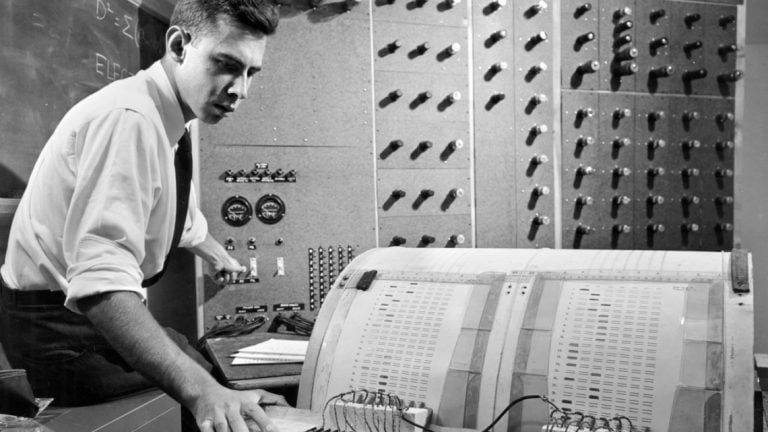
\includegraphics[width=0.8\linewidth]{img/PerceptronRosenblatt}
  \caption{In 1957, Frank Rosenblatt built the Mark I Perceptron at the
  Cornell Aeronautical Laboratory \cite{PARULAMUSTREAD}.}
  \label{RosenPerceptronMKI}
\end{figure}

\subsection{The perceptron algorithm}

Suppose any desired output $Y_j$ for the $j$-th neuron, and for each
iteration $t$ the algorithm follows the operations below:

\begin{align}
  O_j(t) &= \sign\left(\sum^{n}_{k=1} w_k(t) x_{jk}\right)
  \label{eqnOut} \\
  \epsilon_j(t)  &= \frac{\sum_{1}^{n} \left| Y_j - O_j(t) \right|}{N}
  \label{eqnErr} \\
  w_j(t+1) &\longleftarrow w_j(t) - \left(Y_j - O_j(t)\right)r
  \label{eqnWei}
\end{align}

Where Eq. \ref{eqnOut} the output, Eq. \ref{eqnErr} computes the error and
Eq. \ref{eqnWei} the weights update at iteration $t$.

\begin{figure}[!ht]
  \small%
  \centering%
  \begin{tikzpicture}
    \node [term] (st)
      {inicio};
    \node [proc,join] (pr1)
      { Initialize all $w_j$ near to $0$ };
    \node [proc,join] (pr2)
      { Evaluate $O_j$ };
    \node [proc, right=12 of st] (pr3)
      { Update all $w_j$ };
    \node [proc,join]
      { Evaluate $\epsilon_j$ };
    \node [test,join] (cd1)
      { $\epsilon_j \leq \epsilon$};
    \node [term,join]
      {fin};
    \node [coord]                   (rp1) at ($(pr1.east)!0.5!(pr3.west)$) {};
    \node [coord,right = 3 of pr3]  (rp2) {};
    \draw [cong]  (cd1) -| (rp2) -- (pr3);
    \draw [norm]  (pr2) -| (rp1) |- (pr3);
  \end{tikzpicture}
  \caption{Flowchart that describes Rosenblatt's perceptron algorithm.}
  \label{flowchart_perceptron}
\end{figure}

Something important to keep in mind it that it's convergence depends on
that the classes should be linearly separables.


\subsection{Activation, update and error functions}

During this period, and until today, there are different approaches to
neural network implementations trying to optimize it's learning, and
classifying performance.

Adaline (ADAptive Linear Neuron Element) is a neural network developed by
Widrow and Hoff, which was mainly for noise reduction, adaptive filtering,
echo reduction, among other applications. Widrow and Hoff proposed LMS
(Least Mean Squares) algorithm.

About activation functions, there are different activation functions we
can use, such as \textbf{sign}, \textbf{sigmoid}, \textbf{gaussian}, etc.
Also, some functions were defined in the search of the less loss
activation functions such as \textbf{ReLU}.


\section{A perceptrion implementation}


%The implementation will be reported in the complement implemented by
%Quarto \cite{QUARTOWELCOME,QUARTOGUIDE,QUARTODOCUMENTATION}, which you can
%find aside this document.
%
%The code is not optimized in order to get a legible representation of each
%part described here.


%\printbibliography%
